\documentclass{article}

\usepackage{color}     

\usepackage[left=1.25in,top=1.25in,right=1.25in,bottom=1.25in,head=1.25in]{geometry}
\usepackage{amsfonts,amsmath,amssymb,amsthm}
\usepackage{verbatim,float,url,enumerate}
\usepackage{graphicx,subfigure,psfrag}
\usepackage{natbib}
\usepackage{environ}
\usepackage{listings}
\usepackage[dvipsnames]{xcolor}
\usepackage{hyperref}
\usepackage{pifont}     
\usepackage{bbm}

\newtheorem{algorithm}{Algorithm}
\newtheorem{theorem}{Theorem}
\newtheorem{lemma}{Lemma}
\newtheorem{corollary}{Corollary}

\theoremstyle{remark}
\newtheorem{remark}{Remark}
\theoremstyle{definition}
\newtheorem{definition}{Definition}

\newcommand{\argmin}{\mathop{\mathrm{argmin}}}
\newcommand{\argmax}{\mathop{\mathrm{argmax}}}
\newcommand{\minimize}{\mathop{\mathrm{minimize}}}
\newcommand{\maximize}{\mathop{\mathrm{maximize}}}
\newcommand{\st}{\mathop{\mathrm{subject\,\,to}}}
\newcommand{\dist}{\mathop{\mathrm{dist}}}
\newcommand{\minimizewrt}[1]{\underset{#1}{\minimize}}  
\newcommand{\maximizewrt}[1]{\underset{#1}{\maximize}} 
\newcommand{\subjectto}{\mbox{subject to}}            
\newcommand{\ones}{\mathrm 1}                        
\newcommand{\diag}{\mathop{\rm diag}}               
\newcommand{\vecx}{\mathrm{vec}}

\newcommand{\reals}{\mathbb R}
\newcommand{\RR}{\mathbb{R}}
\newcommand{\prox}{\operatorname{prox}}
\newcommand{\dom}{\operatorname{dom}}
\setlength\parindent{0pt}

\def\R{\mathbb{R}}
\def\E{\mathbb{E}}
\def\P{\mathbb{P}}
\def\Cov{\mathrm{Cov}}
\def\Var{\mathrm{Var}}
\def\half{\frac{1}{2}}
\def\sign{\mathrm{sign}}
\def\supp{\mathrm{supp}}
\def\th{\mathrm{th}}
\def\tr{\mathrm{tr}}
\def\dim{\mathrm{dim}}
\def\hbeta{\hat{\beta}}

\lstset{frame=single,
  aboveskip=3mm,
  belowskip=3mm,
  showstringspaces=false,
  columns=flexible,
  basicstyle={\small\ttfamily},
  numbers=none,
  numberstyle=\tiny\color{gray},
  keywordstyle=\color{blue},
  commentstyle=\color{dkgreen},
  stringstyle=\color{mauve},
  breaklines=true,
  breakatwhitespace=true,
  tabsize=3,
  captionpos=b
}
\begin{document}

\title{Homework 4}

\author{\Large Convex Optimization 10-725/36-725}
\date{{\bf Due Friday November 2 at 11:59pm} \\
Submit your work as a single PDF on Gradescope, including the source code.\\
Make sure to prepare your solution to each problem on a separate page.  \\
On Gradescope, please select source code along with the corresponding problem. \\
\textbf{Please choose either Q1 or Q2} ($\text{Score}=\max(\text{Q1},\text{Q2})+\text{Q3}+\text{Q4}$).\\
\bigskip 
Total: 61 points}

\maketitle

\section{Nuclear norm, duality, and matrix completion (17 pts) [Po-wei \& Akash]}

\newcommand{\symm}{\mathbb{S}}

In this problem, we will take a look at convex optimization problems involving \textit{matrix} variables.  We touched on these a little bit in class, and while they might seem somewhat abstract, these sorts of problems are very much connected to real-world applications like Netflix's movie recommendation engine (you are welcome to ask us for further details here).

Let $X \in \reals^{m \times n}$ be a matrix.  The \textit{trace norm} (also known as the \textit{nuclear norm}) of a matrix $X$, which we write as $\| X \|_{\tr}$, can be defined as the sum of the singular values of $X$.

\begin{enumerate}
\item[(a, 5pts)]
Show that computing the trace norm of a matrix, i.e., computing $\| X \|_{\tr}$, can be expressed as the following (convex) optimization problem:
\begin{equation}
\begin{array}{ll}
\maximizewrt{Y \in \mathbb{R}^{m \times n}} & \tr(X^T Y) \\
\subjectto & 
\left[
\begin{array}{cc}
I_m & Y \\
Y^T & I_n
\end{array}
\right]
\succeq 0,
\end{array}
\label{eq:aa:primal}
\end{equation}
where $I_p$ is the $p \times p$ identity matrix.  (By the way, problem \eqref{eq:aa:primal} is a semidefinite program; more on this in part (d) below.)

Hint: recall that the trace norm is the dual of the operator norm; also, think
about using the ``Schur complement'' identity here.  A good reference for this
is Section A.5.5 in the ``Convex Optimization'' book, by Stephen Boyd and
Lieven Vandenberghe. 

\item[(b, 5pts)]
Show that the dual problem associated with \eqref{eq:aa:primal} can be expressed as
\begin{equation}
\begin{array}{ll}
\minimizewrt{\substack{W_{1} \in \symm^{m}, \\ W_{2} \in \symm^{n}}} & \tr(W_{1}) + \tr(W_{2}) \\
\subjectto & 
\left[
\begin{array}{cc}
W_{1} & (1/2) X \\
(1/2) X^T & W_{2}
\end{array}
\right]
\succeq 0,
\end{array}
\label{eq:aa:dual}
\end{equation}
where, just to remind you, $\symm^p$ is the space of $p \times p$ real,
symmetric matrices.

Hint: even though this is a matrix-variate problem, you can just go through the
same steps as if it were a vector-variate problem (form the Lagrangian, maximize
it over the primal variables, etc.)  Recall that a succint way to write the
inner product between matrices $A,B$ is $\tr(A^T B)$ (this is just the usual
inner product, once we unravel them into long vectors).

\item[(c, 2pts)]
Show that the optimal values for problems \eqref{eq:aa:primal} and \eqref{eq:aa:dual} are equal to each other, and that both optimal values are attained.

\item[(d, 5pts)]
In the \textit{matrix completion problem}, we want to find a matrix $X \in \reals^{m \times n}$ of low rank that is close, in a squared error sense, to some observed matrix $Z \in \reals^{m \times n}$.  We do not assume that all of the entries of $Z$ are observed, so we will look at the squared error over $Z$'s observed entries only, which we store in a set $\Omega$ of (observed) row and column indices.  Putting all this together leads us to the following (convex) optimization problem:
\begin{equation}
\begin{array}{ll}
\minimizewrt{X \in \mathbb{R}^{m \times n}} & \sum_{(i,j) \in \Omega} ( X_{ij} - Z_{ij} )^2 + \lambda \| X \|_{\tr},
\end{array}
\label{eq:aa:mtxcomp}
\end{equation}
with tuning parameter $\lambda > 0$.

Show that problem \eqref{eq:aa:mtxcomp} can be expressed as a semidefinite
program (SDP) of the form
\begin{equation*}
\begin{array}{ll}
\minimizewrt{x \in \mathbb{R}^p} & c^T x \\
\subjectto & x_1 A_1 + \cdots + x_p A_p \preceq B,
\end{array}
\end{equation*}
for some fixed $c, B, A_i, \; i=1,\ldots,p$.

Hint: you may start by considering the following constrained problem:
\begin{equation*}
\begin{array}{ll}
\minimizewrt{X \in \mathbb{R}^{m \times n}} & \| X \|_{\tr} \\
\subjectto & \sum_{(i,j) \in \Omega} ( X_{ij} - Z_{ij} )^2 \leq s,
\end{array}
\end{equation*}
which is equivalent to our original penalized problem, for some $s>0$; now you
will probably need to use each of the above parts (in different ways) here to
recast the above in SDP form. 
\end{enumerate}\section{Sparse eigenvectors via the barrier method (17 pts) [Po-Wei]}

In this problem we consider finding a sparse ``eigenvector'' of a matrix $A
\succeq 0$.

\bigskip
\noindent
(a, 1pt) Consider solving the optimization problem
\[
\begin{split}
\max_{x\in\mathbb{R}^n} \;\; & x^TAx \\
\st \;\; & \|x\|_2 = 1 \\
\;\; & \|x\|_1 \le C.
\end{split}
\]
Is this problem convex? Why or why not?

{
\color{blue}
This is not a convex problem. Because the equality constraint $\|x\|_2=1$ is not affine function.
}

\bigskip
\noindent
(b, 1pt) Consider the matrix-variate problem
\[
\begin{split}
\max_{X \in \mathbb{S}^n} \;\; & \tr AX \\
\st \;\; & X \succeq 0 \\
\;\; & \tr X = 1, \\ 
& \mathrm{rank}(X)=1, \\
& \sum_{i,j} |X_{ij}| \le C^2.
\end{split}
\]
Is this problem convex? Why or why not?

{
\color{blue}
This problem is not convex. $rank(X)=1$ is not an affine constraint, and it can't be transformed into convex inequality constraint.
}

\bigskip
\noindent
(c, 4pts) Prove that the problems in parts (a) and (b) are equivalent.  Hint: if
$X$ is rank 1, then we can write it as $X=xx^T$ for some vector $x$.

{
\color{blue}
Because $\mathrm{rank}(X)=1$ and $X\succeq 0$, assume $X=xx^T$ for some vector $x$.
\begin{itemize}
    \item From a. to b.
    \begin{align*}
        \tr AX = \tr Axx^T = x^TA x
    \end{align*}
    \begin{align*}
        \sum_{i,j} |X_{ij}| = \sum_{i,j} |x_i x_j| \le (\sum_i |x_i|)(\sum_j |x_j|) = \|x\|_1^2= C^2
    \end{align*}
    \begin{align*}
        \tr X=\sum_i x_i^2 = \|x\|_2^2 = 1
    \end{align*}
    
    \item From b. to a.
    \begin{align*}
        x^T A x = \tr AX
    \end{align*}
    \begin{align*}
        \|x\|_2=\sqrt{\|x\|_2^2}=\sqrt{\tr X} = 1
    \end{align*}
    \begin{align*}
        \|x\|_1
    \end{align*}
\end{itemize}
}

\bigskip
\noindent
(d, 2pts) Now, consider the matrix-variate problem
\[
\begin{split}
\max_{X \in \mathbb{S}^n} \;\; & \tr AX \\
\st \;\; & X \succeq 0 \\
\;\; & \tr X = 1 \\
& \sum_{i,j} |X_{ij}| \le C^2.
\end{split}
\]
Is this problem convex?  What is the relationship between this problem and that
from part (b)?  

{
\color{blue}
This problem is convex:
\begin{itemize}
    \item The objective function $\tr AX$ is a linear function;
    \item The constraint $X\succeq 0$ is positive semi-definite matrix set, thus convex;
    \item $\tr X=1$ is linear constraint;
    \item $\sum_{i,j} |X_{ij}| \le C^2$ is convex function.
\end{itemize}

The feasible solution for part b must be also feasible for part d. The opposite is not true.
}

\bigskip
\noindent
(e, 4pts) Form the logarithmic barrier for the constraint $\sum_{i,j}|X_{ij}| \le C^2$
and use this along with the logarithmic barrier for $X \succeq 0$ ($\phi(X) =
\log \det X$) to modify the problem in part (d) to have a smooth objective and
equality constraint.

{
\color{blue}
For the constraint $\sum_{i,j}|X_{ij}| \le C^2$, we introduce another set of variables $T_{ij}$ to make it smooth.
\begin{align*}
    &h_1(X,T)=\sum_{ij}T_{ij} - C^2 \leq 0 \\
    &h_2(X,T)=X_{ij}-T_{ij} \leq 0 \\
    &h_3(X,T)=-X_{ij}-T_{ij} \leq 0
\end{align*}

Thus the minimization can be written as:
\[
\begin{split}
\min_{X \in \mathbb{S}^n, T} \;\; & -t\cdot \tr AX -\log (C^2-\sum_{ij}T_{ij}) -\sum_{i,j}(\log (T_{ij}-X_{ij})+\log (X_{ij}+T_{ij}))- \log \det X\\
\st \;\; & \tr X = 1
\end{split}
\]
}

\bigskip
\noindent
(f, 5pts) Setup and describe the iterations of the barrier method for the problem in
part (d), explicitly deriving the Newton update for $X^{(k)}$.

{
\color{blue}
Let $A^a=\mathrm{adj}(A)$, the adjugate matrix of $A$.
\begin{align*}
    &\nabla_{X_{ij}} f = -tA_{ji} - (-\frac{1}{T_{ij}-X_{ij}}+\frac{1}{X_{ij}+T_{ij}})-\frac{A^a_{ji}}{\det A} \\
    &\nabla_{T_{ij}} f = \frac{1}{C^2-\sum_{i,j}T_{ij}} - (\frac{1}{T_{ij}-X_{ij}}+\frac{1}{X_{ij}+T_{ij}})
\end{align*}

\begin{align*}
    &\nabla^2_{X_{ij}X_{pq}}f=
    \begin{cases}
    \frac{1}{(T_{ij}-X_{ij})^2}+\frac{1}{(X_{ij}+T_{ij})^2} ~ & ij=pq \\
    0 & \text{otherwise}
    \end{cases} \\
    &\nabla^2_{T_{ij}T_{pq}}f=
    \begin{cases}
    \frac{1}{(C^2-\sum_{i,j}T_{ij})^2}+\frac{1}{(T_{ij}-X_{ij})^2} + \frac{1}{(X_{ij}+T_{ij})^2} & ij=pq \\
    0 & \text{otherwise}
    \end{cases} \\
    &\nabla^2_{X_{ij}T_{pq}}f=
    \begin{cases}
    -(\frac{1}{(T_{ij}-X_{ij})^2}-\frac{1}{(X_{ij}+T_{ij})^2}) ~ & ij=pq \\
    0 & \text{otherwise}
    \end{cases} \\
    &\nabla^2_{T_{ij}X_{pq}}f=
    \begin{cases}
    -\frac{1}{(T_{ij}-X_{ij})^2} + \frac{1}{(X_{ij}+T_{ij})^2} & ij=pq \\
    0 & \text{otherwise}
    \end{cases}
\end{align*}

Solve the KKT condition with the gradient from $f(x^{(k-1)}$:
\begin{align*}
    \begin{bmatrix}
    \nabla^2 f & A \\
    A & 0
    \end{bmatrix}
    \begin{bmatrix}
    v\\
    w
    \end{bmatrix}
    =\begin{bmatrix}
    -\nabla f \\
     0
    \end{bmatrix}
\end{align*}
Think of the linear constraint $\tr X=1$ as $AX^-=1$, where $X^-$ is a flattened vector.
The next $X$ is:
\begin{align*}
    X^{(k)}=x + tv
\end{align*}
}
\bigskip
\noindent

\section{Second Order Methods for Logistic Regression (22 pts) [Akash]}

In this problem, we will try to classify a viewer's age group from his movie ratings. We formulate the problem as a binary classification with output label  $y \in \{0,1\}^n$, corresponding to whether a person`s age is under $40$, and input features $X \in \mathbb{R}^{n \times (p+1)}$. Similarly to previous homework problems, the first column of $X$ is taken to be $1_n$ to account for the intercept term. We will apply second order methods to solve the logistic regression problem.

We model each $y_i|x_i$ with the probabilistic model
  \[
    \log\left(\frac{p_{\beta}(y_i = 1|x_i)}{1-p_{\beta}(y =
        1|x_i)}\right) = \log\left(\frac{\mu_i}{1-\mu_i}\right) = (X\beta)_i,
  \]
  for $i=1,\ldots,n$, $\beta \in \mathbb{R}^{p+1}$. We use $\beta_0$ to denote the intercept and $\beta_{1:p}$ for the rest of the weights. 

\begin{enumerate}[(a)]
    \item (2 pts) First, show that the negative (conditional) log likelihood (NLL) under the logistic probability model can be expressed as: 
  \[
    l(\beta) = -\sum_{i=1}^{n} \log(p_{\beta}(y_i | x_i)) = -\sum_{i=1}^{n}y_i(X\beta)_i + \sum_{i=1}^{n}\log(1 +
    \exp\{(X\beta)_i\}),
  \]
    Hint: model $y_i|x_i$ as a bernoulli random variable with parameter $\mu_i = p_{\beta}(y_i = 1|x_i)$.
  {
  \color{blue}
  \begin{align*}
      l(\beta)&=-\sum_{i=1}^n\log (p_\beta (y_i|x_i)) \\
      &= -(\sum_{i=1}^n y_i\log (u_i) + (1-y_i)\log (1-u_i)) \\
      &= - \sum_{i=1}^n y_i(\log(u_i)-\log(1-u_i)) - \sum_{i=1}^n\log (1-u_i) \\
      &= - \sum_{i=1}^{n}y_i(X\beta)_i + \sum_{i=1}^n\log \frac{1}{1-u_i} \\
      &= -\sum_{i=1}^{n}y_i(X\beta)_i + \sum_{i=1}^{n}\log(1 + \exp\{(X\beta)_i\})
  \end{align*}
  }
    \item In this part of the problem, we will implement Newton's method for the nonpenalized logistic regression problem and see that in this context, Newton's method is known as Iteratively Reweighted Least Squares (IRLS).
        \begin{enumerate}
    	\item[(i, 1pt)] Express the gradient and the Hessian of the NLL in terms of $X,y,$ and $\mu$.
    	{
    	\color{blue}
    	\begin{align*}
    	    g &= - X^Ty + \sum_{i=1}^n \frac{\exp (X\beta)_i}{1+\exp (X\beta)_i}X_i^T \\
    	    &=-X^Ty + \sum_{i=1}^n \mu_i X_i^T \\
    	    &= -X^T y + X^T \mu \\
    	    &= X^T(\mu-y)
    	\end{align*}
    	\begin{align*}
    	    H(\beta) &= \sum_{i=1}^n\frac{\exp(X\beta)_iX_i^T X_i}{(1+\exp(X\beta)_i)^2} \\
    	    &=\sum_{i=1}^n \mu_i(1-\mu_i) X_i^T X_i \\
    	    &= X^T\diag(\mu_i(1-\mu_i)) X
    	\end{align*}
    	}
    	\item[(ii, 1pt)] Write the Newton update for $\beta$ using the above gradient and Hessian, using $t$ to denote step-size.
    	{
    	\color{blue}
    	\begin{align*}
    	    \beta^+=\beta - t H^{-1}g
    	\end{align*}
    	}
    	
    	\item[(iii, 1pts)] Show that the Newton update has the form of a weighted least-squares estimation problem. This is why in this context, Newton's method is known as IRLS.
    	
    	{
    	\color{blue}
    	For convinience let $D = \diag(\mu_i(1-\mu_i))$
    	Let:
    	\[
    	f(\beta)=(z-X\beta)^T tD(z-X\beta)
    	\]
    	where $z= X\beta^{k-1}-tD^{-1}(\mu-y)$
    	\begin{align*}
    	    \nabla f = -tX^TD(z-X\beta)=0
    	\end{align*}
    	then
    	\begin{align*}
    	    \beta^\star &= (X^TDX)^{-1}X^T D z \\
    	    &=(X^TDX)^{-1}X^T D X\beta - t(X^TDX)^{-1}X^T D D^{-1}(\mu-y) \\
    	    &=\beta - t H^{-1}X^T(\mu-y) \\
    	    &=\beta - t H^{-1}g
    	\end{align*}
    	As we see here, the optimal solution of IRLS objective $f(\beta)$ has the same form as the Newton update.
    	}
    	\item[(iv, 1pts)] Given $X$ and $y$, write out the steps for performing IRLS to estimate $\hat{\beta}$. Assume a fixed step size $t$ in the steps.
    	{
    	\color{blue}
    	\begin{enumerate}
    	    \item[1.] Initialize $\beta$;
    	    \item[2.] If the convergence requirement is satisfied, return $\beta$;
    	    \item[3.] Compute gradient and Hessian:
    	    \begin{align*}
    	        &\mu=\frac{1}{1+\exp(-X\beta)} \\
    	        &D=\diag(\mu_i(1-\mu_i)) \\
    	        &g = X^T(\mu-y) \\
    	        &H = X^T DX
    	    \end{align*}
    	    \item[4.] Compute next $\beta^+$:
    	    \begin{align*}
    	        \beta^+=\beta - t H^{-1}g
    	    \end{align*}
    	    \item[5.] Go to step 2.
    	\end{enumerate}
    	}
        \item[(v, 3pts)] Now, implement IRLS with backtracking using the movie data set on the website (in \texttt{hwk4\_gs3.zip}, for this homework, not the second one). Initialize your weights with zeros. Use $\alpha = 0.01$ and shrink parameter $\beta = 0.9$ for backtracking. You can stop IRLS when the change between consecutive objective values is less than 1e-6. Report both the train and test errors of classifying whether a person is under $40$. Plot $f^{(k)} - f^{\star}$ versus $k$,  where $f^{(k)}$ denotes the objective value at outer iterations $k$ of IRLS, and the optimal objective value is $f^\star = 186.637$ on a semi-log scale (i.e. where the y-axis is in log scale).
        {
        \color{blue}
        
        See Fig \ref{fig:irls}.
        \begin{figure}
            \centering
            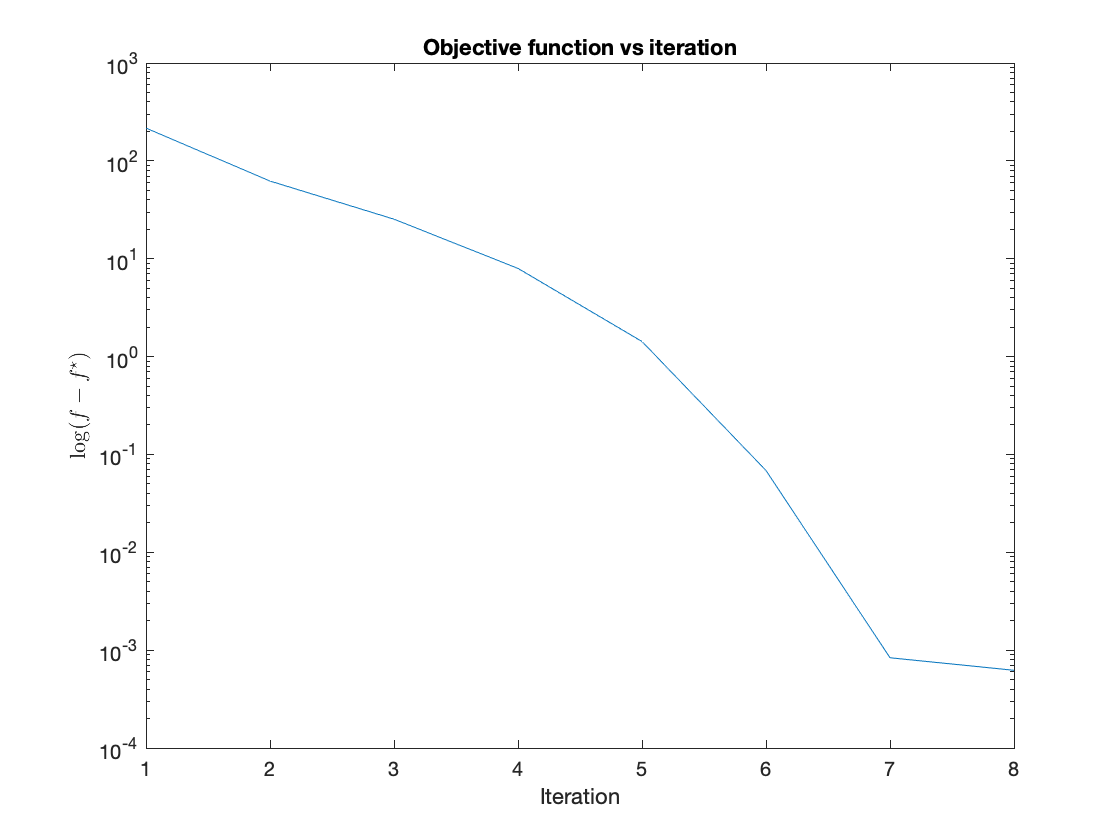
\includegraphics[scale=.3]{irls.png}
            \caption{IRLS}
            \label{fig:irls}
        \end{figure}
        
        Train error: 0.1583;
        
        Test error: 0.2952.
        }
        \end{enumerate}

    \item Now, we introduce regularization to the NLL to improve our test error. The problem becomes:
    \begin{equation}
		\min_{\beta \in \mathbb{R}^{p+1}} \quad l(\beta) + \lambda\|\beta_{1:p}\|_1
	\label{eq:penalty}
	\end{equation}
	    \begin{enumerate}
	    \item[(i, 2pts)] Rewrite \eqref{eq:penalty} as a problem that has a smooth criterion, aims to preserve the sparsity of the original problem, and can be solved by an interior point method. (Hint: consider introducing a new variable and corresponding inequality constraints).
	    {
	    \color{blue}
	    
	    As usual, the absolute value term can be changed into smooth function with new variables $\xi\in \mathbb{R}^p$.
	    \begin{align*}
	        \min_{\beta \in \mathbb{R}^{p+1},\xi \in \mathbb{R}^p} \quad &l(\beta) + \lambda\sum_{i=1}^p \xi_i \\
	        s.t. &\xi_i\geq \beta_i \\
	             &\xi_i\geq -\beta_i
	    \end{align*}
	    }
	    \item[(ii, 3pts)] Describe the iterations of the barrier method for the problem in (i), explicitly deriving the Newton updates.
	    {
	    \color{blue}
	    
	    Let the logrithmetic barrier objective function
	    \[F=t(l(\beta) + \lambda\sum_{i=1}^p \xi_i)-\sum_{i=1}^p(\log(\xi_i-\beta_i))+\log(\xi_i+\beta_i))\]
	    $F = t(l(\beta) + \lambda\sum_{i=1}^p \xi_i)-$. We have:
	    \begin{align*}
	        g_F =
	        \begin{pmatrix}
	        g_0 \\
	        g_i + \dfrac{1}{\xi_i-\beta_i} - \dfrac{1}{\xi_i+\beta_i}\\
	        \lambda \mathbf{1} - \dfrac{1}{\xi_i-\beta_i} - \dfrac{1}{\xi_i+\beta_i}\\
	        \end{pmatrix}
	    \end{align*}
	    \begin{align*}
	        H_F =
	        \begin{bmatrix}
	        H &  \\
	         & \mathbf{0}_{p\times p} \\
	        \end{bmatrix}+
	        \begin{bmatrix}
	        0 & &\\
	         & \diag(\dfrac{1}{(\xi_i-\beta_i)^2}+\dfrac{1}{(\xi_i+\beta_i)^2}) & \\
	         & & \diag(\dfrac{1}{(\xi_i-\beta_i)^2}+\dfrac{1}{(\xi_i+\beta_i)^2}) \\
	        \end{bmatrix}
	    \end{align*}
	    Newton update:
	    \begin{align*}
	        \begin{pmatrix}
	        \beta \\
	        \xi \\
	        \end{pmatrix}^+ = 
	        \begin{pmatrix}
	        \beta \\
	        \xi \\
	        \end{pmatrix} - t (H_F)^{-1}g_F
	    \end{align*}
	    }
	    \item[(iii, 4pts)] Implement the barrier method described above. For the barrier parameters $t$(the multiplier for the original criterion in \eqref{eq:penalty}) and $\mu$(the constant by which $t$ increases at each outer iteration of the barrier method), use $\mu=20$ and start with $t=5$. A good number for $m$(the constant that, together with $t$, bounds the duality gap) is the number of constraints in the barrier problem. For backtracking during the Newton method steps, use $\alpha=0.2$ and $\beta=0.9$. You can use 1e-9 as the stopping threshold for both the Newton method and the barrier method. Remember to initialize the centering Newton method step with a strictly feasible point (hint: in MATLAB, one simple way to find such a point is with $linprog$).
    
	    Use the barrier method with $\lambda=15$ to classify whether a viewer is under $40$. Report the train and test classification errors. Report the number of zeros at the solution $\beta^{\star}$. Here we consider any number with absolute value under 1e-10 to be zero.
	    
	    \item[(iv, 4 pts)] Now, implement proximal gradient descent with backtracking for logistic regression with lasso penalty. You can refer back to the group lasso problem in homework 2 to help you in your implementation.

      Using $\lambda=15$, run proximal gradient descent (with backtracking line search, with shrinkage parameter $\beta=0.5$) on the training data.
	    
	    To compare the convergence of both the barrier method and the proximal gradient descent, plot $f^{(k)} - f^{\star}$ versus $k$,  where $f^{(k)}$ denotes the objective value at total number of iterations $k$ of the algorithms, and the optimal objective value is $f^\star = 306.476$ on a semi-log scale (i.e. where the y-axis is in log scale). Plot these in the same figure. 

      To be clear, when counting total number of iterations, each backtracking iteration counts as 1 iteration (for prox gradient descent), and each inner Newton iteration counts as 1 iteration (for log-barrier method).
	    \end{enumerate}
\end{enumerate}

\textbf{Attach all relevant code to the end of this problem.}
\section{Interior Point Methods for SVMs [Wenbo] (22 pts)}

\paragraph{Overview} In this question we will continue playing with the same kernel support vector machine as we did in last homework. Recall that in homework 3 we have developed the dual optimization problem for support vector machine with radial basis function (RBF) kernel, and solved it using standard QP solver. This time, we will write our own solver, and solve the kernel-SVM using the
barrier method and the primal-dual interior point method.

Following homework 3, we will be using the same dataset with inputs $X \in \mathbb R^{863 \times 2}$ and labels $y \in \{-1, 1\}^{863}$ from \texttt{data.txt} on the class website.

\paragraph{Kernel SVM} Recall from homework 3, the primal optimization of
kernel SVM is
$$
\begin{aligned}
& \underset{\beta, \xi_i}{\text{minimize}} && \frac{1}{2}||\beta||_2^2 + C\sum_{i=1}^n\xi_i\\
& \text{subject to} && y_i(\beta^T\phi(x_i) + \beta_0) \geq 1-\xi_i & i = 1,\ldots, n\\
& && \xi_i \geq 0 & i = 1,\ldots, n
\end{aligned}
$$
where $\xi_1, \ldots, \xi_n$ are the slack variables. This is equivalent to solving the following dual optimization problem
\begin{equation}
\label{eq:dual}
\begin{aligned} 
  & \underset{w}{\text{maximize}} && 1^Tw - \frac{1}{2}w^T \tilde{K}w \\
  & \text{subject to} && 0\leq w\leq C1, \quad w^Ty = 0\\
\end{aligned}
\end{equation}
where $w$ is the dual variable, $K_{ij} = \langle\phi(x_i), \phi(x_j)\rangle$, and $\tilde{K}_{ij} = y_iy_jK_{ij}$.

Again, recall that the support vectors correspond to the instances with the dual
variable $w_i > 0$.
The optimal primal vector
$\beta^*$ can be represented in terms of the dual optimal $w^*_i, i=1,\ldots, n$ as
$\beta^* = \sum_{i=1}^n w^*_iy_i\phi(x_i)$.
To solve for $\beta^*_0$ from the
dual, we can pick any instance $j$ that lies on the margin, and compute
$\beta^*_0$ as 
$$\beta^*_0 = y_j - (\beta^*)^T\phi(x_j) = y_j - \sum_{i=1}^n w_i^* y_iK_{ij}$$
In practice, in order to reduce the variance, we can take the average as
\begin{align}
\beta^*_0 = \frac{1}{|J|}\sum_{j\in J}\left(y_j - \sum_{i=1}^n w_i^* y_iK_{ij}\right)
\label{eq:kernel_svm_intercept}
\end{align}
where $J$ is the set of instances on the margin.

Lastly, the prediction for a given vector $x\in\R^d$ can be
calculated as follows:
\begin{equation}
  \hat{y} = \sign\left(\sum_{i=1}^n w^*_i y_i \langle \phi(x), \phi(x_i)\rangle + \beta^*_0\right) = \sign\left(\sum_{i=1}^n w^*_i y_i K(x, x_i) + \beta^*_0\right)
  \label{eq:kernel_svm_prediction}
\end{equation}

The RBF kernel is expresses as
$$\langle \phi(x_i), \phi(x_j) \rangle = K_{ij} = \exp\left(-\gamma||x_i - x_j||_2^2\right)$$
where we fix $\gamma = 500$.

\textbf{Please submit your code as an appendix to this problem}.

\begin{enumerate}[(a)]

\item \textbf{Barrier Method} 
  \begin{enumerate}[(i)]

  \item[(i, 5pts)] Derive the gradient and the Hessian of the dual criterion $f(w)$, and of
    the log barrier objective of the form $tf(w) + g(w)$, where $g(w)$ is the
    log barrier term which takes the role of the inequality constraint. (Note,
    the equality constraint remains unchanged in the log barrier problem!)
    Confirm that the Hessian only changes from that of the original version in
    the diagonal entries. (Hint: This may be helpful in understanding the update
    directions in the interior point implementation in part (b).)
    
    {
    \color{blue}
    The dual is:
    \begin{equation*}
    \begin{aligned} 
      & \underset{w}{\text{minimize}} && \frac{1}{2}w^T \tilde{K} w -1^Tw \\
      & \text{subject to} && 0\leq w\leq C\mathbf{1}, \quad w^Ty = 0\\
    \end{aligned}
    \end{equation*}
    The gradient and Hessian:
    \begin{align*}
        \nabla f(w) = \tilde{K} w-\mathbf{1}
    \end{align*}
    \begin{align*}
        \nabla^2 f(w) = \tilde{K}
    \end{align*}
    The log barrier term $g(w)$:
    \begin{align*}
        g(w) = -\sum_{i=1}^n \log (C-w_i)-\sum_{i=1}^n\log w_i
    \end{align*}
    Gradient and Hessian of the log barrier objective $F(w)=tf(w)+g(w)$:
    \begin{align*}
        \nabla_i F= t(\tilde{K_{i\cdot}}w-1)+\frac{1}{C-w_i}-\frac{1}{w_i}
    \end{align*}
    \begin{align*}
        &\nabla_{ii} F=t\tilde{K}_{ii}+\frac{1}{(C-w_i)^2}+\frac{1}{w_i^2} \\
        &\nabla_{ij} F=t\tilde{K}_{ij} ~ i\neq j
    \end{align*}
    
    As we can see, the Hessian of the log barrier objective $F$ only changes the $\nabla_{ii}F$, the diagonal entries (ignoring the constant $t$).
    }
    
  \item[(ii, Bonus question, 5pts)] Implement the barrier method as described in
    class to solve the SVM dual. Note, you will be using an equality-constrained
    Newton method with backtracking, in the barrier method updates. Set $C=0.1$. Using
    initial $t=10000$ and $\mu=4$, run your barrier method until
    $m/t < 10^{-8}$. For the inter Newton centering step, run until the Newton decrement $\tfrac1{2} \lambda(x)^2 < 10^{-16}$.
    
    Several steps you should address:
    \begin{enumerate}[1)]
      \item Describe how to obtain an initial feasible point in our problem.
      \item Describe how to obtain the equality-constrained Newton update
        direction.
      \item Describe the stopping rule for in terms of the Newton decrement,
        using the equality-constrained Newton direction update. Note, your
        stopping criterion should be sufficiently small, for your inner Newton
        to have good precision.
      \item Describe how to find an initial step size prior backtracking
        step. (Hint: the key is to choose a step size that would allow the
        upcoming update to be feasible; there are several ways to do this.)
      \item For backtracking line search, you can use $\alpha = 0.01$ and
        $\beta = 0.5$, per notation in the lecture notes.
    \end{enumerate}
    Plot the objective value versus iterations.
    Report the optimal objective value at the optimal training weights $w^*$:
    $f^* = \frac{1}{2}(w^*)^T\tilde{K}w^* - 1^Tw^*$. Report the number of
    support vectors, considering only $w^* > 10^{-5}$. Use the optimal
    $w^*$ to do prediction, report classification accuracy. A good
    check is to see if your answer agrees with (b) (or with standard QP solver).
  \end{enumerate}




\item \textbf{Primal-Dual Interior Point Method}
  \begin{enumerate}[(i)]
      \item[(i, 2pts)] For a given $t > 0$, list the perturbed KKT condition for this problem.
      
      {
      \color{blue}
      
      With the notation from ii., the Lagragian for the original problem (without log barrier) is:
      \begin{align*}
          L = \frac{1}{2}w^T \tilde{K} w - w^T \mathbf{1} + \lambda y^T w + (-w^T)u + ((w-C\mathbf{1})^T)v
      \end{align*}
      Perturbed KKT conditions:
      \begin{align*}
          \begin{cases}
          \frac{\partial L}{\partial w}=\tilde{K}w-\mathbf{1}+\lambda y-\mu +v = 0 \\
          y^T w = 0 \\
          -\diag (w)u + \frac{1}{t}\mathbf{1} = 0 \\
          -\diag (C\mathbf{1}-w)v + \frac{1}{t}\mathbf{1} = 0 \\
          w-C\mathbf{1}\leq 0 \\
          -w \leq 0 \\
          \lambda \geq 0 \\
          u\geq 0 \\
          v\geq 0
          \end{cases}
      \end{align*}
      }

        \item[(ii, 2pts)] Let $u_i \geq 0$ be the dual variable correspond to the inequality constraint $-w_i \leq 0, \forall i$ and $v_i\geq 0$ be the dual variable correspond to the inequality constraint $w_i\leq C, \forall i$. Let $\lambda$ be the dual variable correspond to the equality constraint $y^Tw = 0$. Write down the expression for the primal residual $r_{\text{prim}}$, the dual residual $r_{\text{dual}}$ and the centrality residual $r_{\text{cent}}$.
        
        {
        \color{blue}
        \begin{align*}
            &D_u h(w) = 
            \begin{bmatrix}
            \nabla h_1(w)^T \\
            \cdots \\
            \nabla h_m(w)^T
            \end{bmatrix} = 
            -I \\
            &D_v h(w) = I
        \end{align*}
        \begin{align*}
            &r_{dual} = \nabla f(w) + Dh_u(w)^T u + Dh_v(w)^T v + y\lambda = \nabla f(w) - u + v + \lambda y \\
            &r_{cent} = -\diag(u)h_u(w)-\diag(v)h_v(w)-\frac{1}{t}\mathbf{1}=\diag(u)w-\diag(v)(w-C\mathbf{1})-\frac{1}{t}\mathbf{1} \\
            &r_{prim} = y^T w
        \end{align*}
        }

        \item[(iii, 2pts)] Define the residual vector $r(w, u, v, \lambda) = (r_{\text{dual}}, r_{\text{cent}}, r_{\text{prim}})$ and $z = (w, u, v, \lambda)$. The primal-dual interior point method is trying to find an update direction $\Delta z = (\Delta w, \Delta u, \Delta v, \Delta\lambda)$ such that $r(z + \Delta z) = 0$. However, in general $r(z + \Delta z) = 0$ corresponds to a system of nonlinear equations that does not admit closed-form solution, so instead we make a first-order approximation to $r(z + \Delta z)$ and solves the corresponding linear system: $r(z + \Delta z)\approx r(z) + Dr(z)\Delta z = 0$. Write down the linear system to be solved in order to get $\Delta z$. $\Delta z$ is also known as the Newton direction.
        
        {
        \color{blue}
        
        First let's compute something.
        \begin{align*}
            \nabla^2 f(w) + \sum_{i=1}^n u_i\nabla^2 hu_i(w) + \sum_{i=1}^n v_i \nabla^2 hv_i(w) = \nabla^2 f(w)
        \end{align*}
        \begin{align*}
            \begin{bmatrix}
            \nabla^2 f(w) & D_u h(w)^T & D_v h(w)^T & y \\
            -\diag(u) D_uh(w) & -\diag(h_u(w)) & 0 & 0 \\
            -\diag(v) D_vh(w) & 0 & -\diag(h_v(w)) & 0 \\
            y^T & 0 & 0 & 0
            \end{bmatrix}
            \begin{pmatrix}
            \Delta w \\
            \Delta u \\
            \Delta v \\
            \Delta \lambda
            \end{pmatrix}
            =-\begin{pmatrix}
            \nabla f(w) - u + v + \lambda y \\
            -\diag(u)  h_u(w) - \frac{1}{t}\mathbf{1} \\
            -\diag(v) h_v(w) - \frac{1}{t}\mathbf{1} \\
            y^T w
            \end{pmatrix}
        \end{align*}
        which is
        \begin{align*}
            \begin{bmatrix}
            \tilde{K} & -I & I & y \\
            \diag(u) & \diag(w) & 0 & 0 \\
            -\diag(v) & 0 & -\diag(w-C\mathbf{1}) & 0 \\
            y^T & 0 & 0 & 0
            \end{bmatrix}
            \begin{pmatrix}
            \Delta w \\
            \Delta u \\
            \Delta v \\
            \Delta \lambda
            \end{pmatrix}
            =-\begin{pmatrix}
            \tilde{K}w - \mathbf{1} - u + v + \lambda y \\
            \diag(u)w - \frac{1}{t}\mathbf{1} \\
            -\diag(v) (w-C\mathbf{1}) - \frac{1}{t}\mathbf{1} \\
            y^T w
            \end{pmatrix}
        \end{align*}
        }

    \item[(iv, 2pts)]   Primal-dual interior point method requires a strictly feasible point of (\ref{eq:dual}) as a start point. Form a linear program that can be used to find such a strictly feasible initial point.

    {
    \color{blue}
    The linear program to find strictly feasible point is:
    \begin{align*}
        y^T w = 0, 0< w < C\mathbf{1}
    \end{align*}
    Suppose $y$ vector has $n_p$ number of 1 and $n_n$ number of -1. Let $0 < q_n = C/2\min\{n_p/n_n,1\} < C$, $0< q_p = q_nn_n/n_p < C$. We then let $w_i=q_p$ where $y_i=1$ and $w_i=q_n$ where $y_i=-1$. Thus $y^Tw=q_pn_p - q_nn_n=0$ and $0<w_i<C$.
    }
    \item[(v, 9pts)]   Implement the primal-dual interior point method to solve the minimization problem you formed in (i). We fix $C = 0.1$, $\mu = 1000$. You should stop your algorithm when both the following two conditions are met:
        \begin{itemize}
          \item   $(||r_{\text{prim}}||_2^2 + ||r_{\text{dual}}||_2^2)^{1/2}\leq 10^{-6}$.
          \item   The surrogate duality gap is less than or equal to $2\times 10^{-6}$.
        \end{itemize}
      Here is a list of tips that might be helpful to you:
      \begin{itemize}
          \item   Use the LP formed in the last question to find a strictly feasible initial point.
          \item   After obtaining each Newton direction, it is important to compute a corresponding step size such that both the primal and the dual variables are feasible. 
          \item   For backtracking line search, you can use $\alpha = 0.01$ and $\beta = 0.5$ (Note this $\beta$ corresponds to the parameter to shrink the step size, not the $\beta$ in the primal SVM).
          \item   It is important to tune to barrier parameter $\mu$ such that your algorithm stops within a fair amount of iterations. As a reference, the TA's implementation stops in $99$ iterations.
      \end{itemize}
      Plot the objective value versus iterations.
      Report the function value at the optimal $w^*$: $f^* = \frac{1}{2}(w^*)^T\tilde{K}w^* - 1^Tw^*$. Report the number of support vectors. Here we consider any $w^*$ that is less than $10^{-5}$ to be $0$. Use the optimal $w^*$ to do prediction and report classification accuracy. 
      
      {
      \color{blue}
      It may not be wise to throw the above equations directly into MATLAB and solve the update step. Let's first simplify it.
      
      First we can solve the $\Delta u$.
      \begin{align*}
          &\diag (u) \Delta w + \diag (w) \Delta u = -\diag(w)u+\frac{1}{t}\mathbf{1} \\
          \Rightarrow &\Delta u = -u+\frac{1}{t}\diag(\frac{1}{w_i})\mathbf{1} -\diag(\frac{u_i}{w_i})\Delta w
      \end{align*}
      
      Then solve $\Delta v$:
      \begin{align*}
      &-\diag(v)\Delta w + \diag(C\mathbf{1}-w)\Delta v = -\diag(C\mathbf{1}-w)v + \frac{1}{t}\mathbf{1} \\
      \Rightarrow & \Delta v = -v+\frac{1}{t}\diag(\frac{1}{C-w_i})\mathbf{1}+\diag (\frac{v_i}{C-w_i})\Delta w
      \end{align*}
      
      Then solve $\Delta \lambda$.
      
      We now have:
      \begin{align*}
          &\tilde{K} \Delta w - \Delta u + \Delta v + y\Delta \lambda = -(\tilde{K}w - \mathbf{1} - u + v + \lambda y) \\
          &y^T\Delta w=y^T w \\
          &\Delta u = -u+\frac{1}{t}\diag(\frac{1}{w_i})\mathbf{1} -\diag(\frac{u_i}{w_i})\Delta w \\
          &\Delta v = -v+\frac{1}{t}\diag(\frac{1}{C-w_i})\mathbf{1}+\diag (\frac{v_i}{C-w_i})\Delta w
      \end{align*}
      Let:
      \begin{align*}
          &G=\diag(\frac{u_i}{w_i}+\frac{v_i}{C-w_i}) \\
          &Q = \tilde{K}+G \\
          &z = -\tilde{K}w + \mathbf{1}-\lambda y + \frac{1}{t}\diag(\frac{1}{w_i}-\frac{1}{C-w_i})\mathbf{1}
      \end{align*}
      then we have:
      \begin{align*}
          \Delta \lambda = \frac{y^TQ^{-1}z + y^T w}{y^T Q^{-1} y}
      \end{align*}
      Finally solve $\Delta w$.
      We now have:
      \begin{align*}
          &\tilde{K} \Delta w - \Delta u + \Delta v + y\Delta \lambda = -(\tilde{K}w - \mathbf{1} - u + v + \lambda y)
      \end{align*}
      Then we have:
      \begin{align*}
          \Delta w = Q^{-1}(z-y\Delta \lambda)
      \end{align*}
      
      The objective value versus iterations:
      \begin{figure}
          \centering
          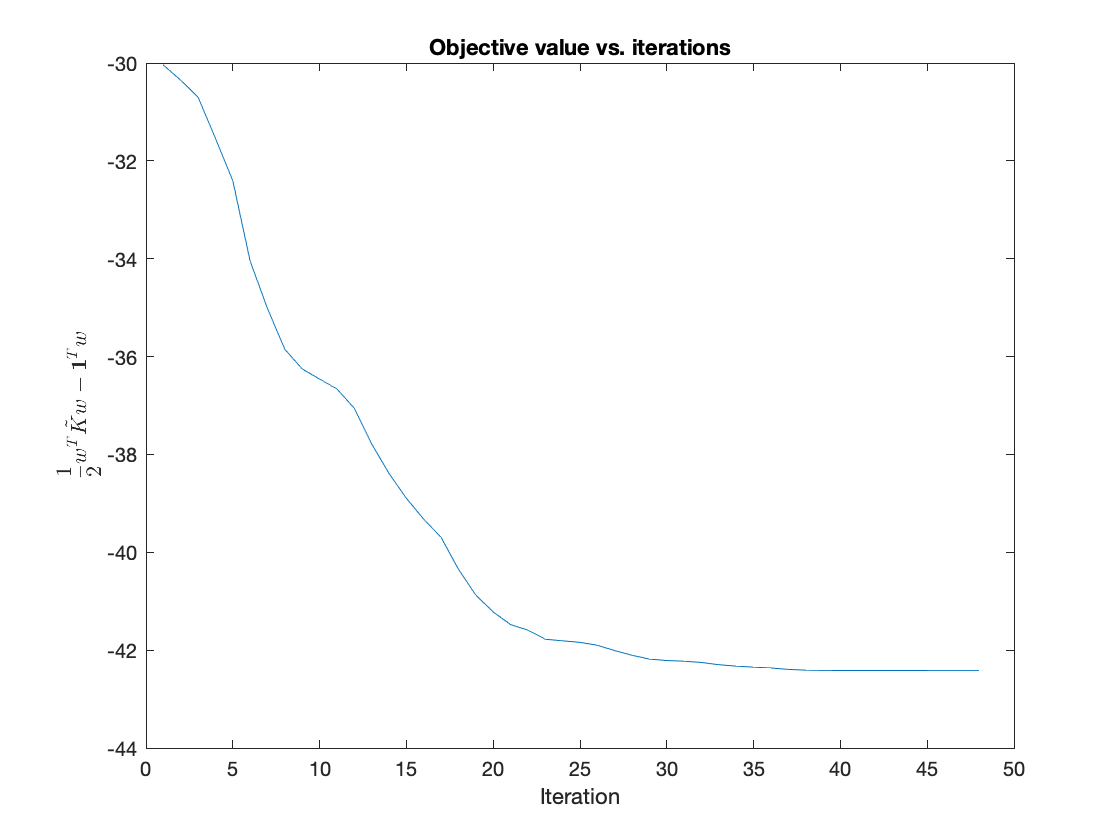
\includegraphics[scale=.4]{obj_barrier.png}
          \caption{Objective function versus iterations}
          \label{fig:my_label}
      \end{figure}
      
      The function value at optimal $w^\star$ is -42.417465.
      
      The number of S.V.: 745.
      
      Classification error: 0.0012; false positive: 0.0026, false negative: 0.
      }
  \end{enumerate}

\end{enumerate}

\textbf{Please submit your code as an appendix to this problem.}

\end{document}
